\documentclass[../full_thesis/full_thesis.tex]{subfiles}

% Default image directory
\graphicspath{{../introduction/img/}} 
\newcommand{\IntroductionDir}{../introduction}

\begin{document} 

The story of a \emph{neutron star} (NS) begins with the death of a main-sequence star
in a supernova event. Prior to this, the nuclear fusion of hydrogen atoms into
helium provides pressure supporting the star in an equilibrium configuration
with the inward pressure of the stars self-gravity. Eventually the star depletes
its reserves of hydrogen and can no longer maintain the equilibrium. If the
star has an initial mass greater than $\sim 8 \Msun$, then it may undergo a
\emph{core-collapse supernova} during which the temperatures and pressure rapidly
increase. Under these conditions the electrons and protons undergo inverse
beta decay combining to form neutrons and neutrinos
\begin{equation}
    e^{-} + p \rightarrow n + \nu.
\end{equation}
Once the pressures reaches nuclear densities, neutron degeneracy pressure can
halt the collapse in a new equilibrium configuration; the resulting remnant is
a neutron star. However, if the remnant has a mass greater than $\sim 5 \Msun$,
neutron degeneracy pressure will be unable to support the gravitational
pressure and it will collapse to form a black hole.

The idea of neutrons stars was first postulated by Landau as `dense stars
which look like giant atomic nuclei' \citep{Yakovlev2013} even before the
discovery of the neutron by \citep{Chadwick1932}. However it was
\citet{Baade1934} who made the explicit prediction of a neutron star whilst
trying to explain the energy released in supernova explosions.

The maximum radius such a star can support is $\sim 10$~km but the mass
compressed into this volume is $\sim M_{\odot}$.  They can rotate with
frequencies up to 700~Hz and exist as either \emph{isolated} or as part of a
binary system.  In either of these systems their compactness means they are
potential sources of detectable gravitational waves. In fact the orbital decay
of the binary neutron star system PSR~1913+16 discovered by \citet{Hulse1975}
and subsequently analysed by \citet{Taylor1982} provided the first evidence for
gravitational waves.  NSs can have extreme magnetic fields with estimates
strengths up to $10^{15}$ gauss. 

Our knowledge of neutron stars is founded on observing them in the variety of
system detectable by astronomy. In this thesis we will investigate how we can
use current electromagnetic observations to further our understanding of neutron
star physics by investigating the causes of so-called \emph{timing-noise}.
Detecting gravitational waves from isolated neutron stars will provide a second
channel to investigate neutron star physics; in this thesis I will also
investigate the importance timing-noise and glitches may have on the ability to
detect such gravitational waves.

In this introductory chapter, we will describe current understanding of neutron
stars concentrating on those observed as 'pulsars'. The basic astrophysics will
be introduced along with the methods used to collect data. Finally we will describe
two phenomena, glitches and timing-noise, which provide an opportunity to
probe the neutron star physics.


\section{Observation of pulsars and their identification with neutron stars}
After the conception of neutron stars as stable compact objects there was
thought to be little chance of observing them. They are many orders of
magnitude smaller than other celestial objects and soon after their formation
in rare supernovae events (the last observed event took place in 1604 and was
observed by Johannes Kepler) they are rapidly cooled by the emitted neutrinos
making their thermal emission difficult to detect.

In 1968 a bright periodic EM signal, now known as PSR~B1919+21, was identified
by \citet{Hewish1968} during a high time-resolution survey for interplanetary
scintillation. The source was measured with a radio radio frequency of 81.5~MHz
and pulsed with a period of $\sim 1.377$~s; this led to the name \emph{pulsars}
to refer to such sources.  Following this, several other similar objects where
discovered. A unifying feature of all pulsars is the clock-like stability of
the pulsations - something not rivalled by any other astrophysical phenomenon.
This stability indicates that the source must be a coliminated beam fixed to a
rotating body such that, as it rotates, the beam sweeps out like a lighthouse;
in this way the pulsation period is exactly the rotation period of the body.
Alternative models such as emission due to accretion from a binary companion
could never reach the stability's seen in pulsars.

For any rotating body to remain gravitationally bound, its rotation frequency is
constrained by the requirement that the centrifugal acceleration at the equator
be less than the gravitational acceleration. The rotation frequency of the observed
pulsars ruled out all known astrophysical bodies except the two most compact
objects, neutron stars and black holes, since all other bodies would not be
gravitationally bound at these frequencies. Isolated black holes are unable to
support an electromagnetic emission mechanism, this left only neutron stars
as candidates.

The identification of pulsars with neutron stars came independently from
\citet{Pacini1967} and \citet{Gold1968}. They suggested that a rapidly rotating
neutron star with a strong dipolar magnetic field would stream radiation out
along the magnetic axis. If this axis is misaligned from the rotation axis,
then the beams are swept out like a lighthouse. Beams passing over the earth
are observed as periodic pulses at the rotation frequency of the star.  Such a
model predicts that the electromagnetic radiation should exert a torque and
slow-down the rotation.  This slowdown was subsequently measured in the Crab
pulsar, which was discovered at the centre of the Crab nebulae which is a
supernova remnant, agreeing with the prediction of \citet{Baade1934}.

These early detection gave birth to a new field of astronomy: pulsar astronomy.
Since then, the field has detected over 2000 radio pulsars, measured thermal
emission from a handful of nearby neutron stars with typical temperatures of
$10^{5}$K to $10^{6}$K \citep{pavlov2003thermal}, found neutron stars in
accreting binary systems with companions, and identified many other ways to
observe neutron stars. We will discuss some of these which are relevant to this
thesis in Sec.~\ref{sec: categorising neutron stars}, but first in
Sec.~\ref{sec: pulsar timing methods} we describe the techniques used by the
field to identify and `time' radio pulsars.


\section{Categorising neutron stars}
The timing properties, and other features measured by the timing model, for
over 2000 pulsars observed can be accessed via the ATNF pulsar catalogue
\citep{ATNF}.  We can categorise the population by their measured values of
period $P$ and period derivative $\Pdot$. This is done by plotting them in a
so-called $P - \Pdot$ diagram as shown in Fig.~\ref{fig: Period_PeriodDot}.
Some of the pulsar varieties have been marked in this plot and we now discuss
their features.

\begin{figure}[hb]
    \centering
    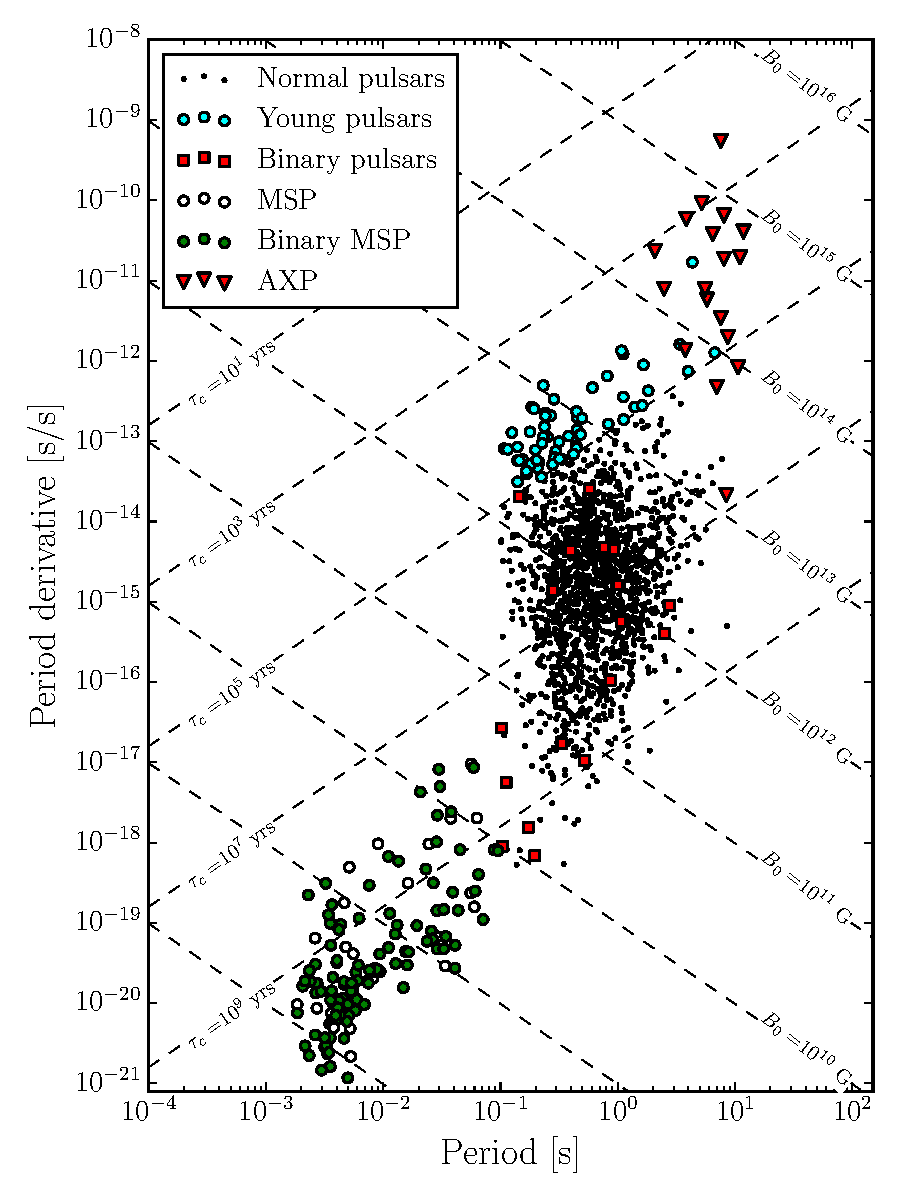
\includegraphics[width=0.8\textwidth]{Period_PeriodDot}
    \caption{Period - period diagram using data taken from the ATNF pulsar
             catalogue \citep{ATNF}. Dashed lines show inferred magnetic fields
             and characteristic ages as described in Sec.~\ref{sec: rotation
             powered pulsars}}
    \label{fig: Period_PeriodDot}
\end{figure}

The majority of pulsars, referred to as the `normal' pulsars, are
\emph{isolated} (without a binary companion) and have typical periods of
$P=10^{-1}-10^{1}$~s. These can be described as \emph{rotation powered} pulsars
since the EM radiation is powered by the loss of rotational energy. As
described later in Sec.~\ref{sec: rotation powered pulsars}, estimates can be made
for their characteristic age $\tau_{c}$ and surface magnetic field strength
$B_{0}$ based on a dipole spin-down model. Constant lines of these quantities
are plotted in Fig.~\ref{fig: Period_PeriodDot}. Of the normal pulsars, we
can identify the young pulsars as those for which $\tau_{c}<10^{5}$~yrs. Some
of these, such as the Crab and Vela, can be directly associated with their
supernova remnant from which they were formed \citep{Kaspi1996}.

A second smaller population of isolated rotation powered pulsars exists with
$P<10^{-1}$~s, these are the \emph{millisecond pulsars} (MSPs). These special
class of pulsars are believed to start life as normal pulsars, but are then
spun-up through accretion from a normal star. In support of this hypothesis,
the majority of MSPs in figure \ref{fig: Period_PeriodDot} have a binary
companion \citep{wijnands1998millisecond}.  During the accretion stage, the
mechanism responsible for the electromagnetic emission is thought to switch-off
and so we do not see their pulsations. However, we can observe them in an X-ray
binary when they undergo outburst \citep{lewin1997x}; this is caused by the
heating of material in the accretion disk as the neutron star draws material
from the companion star.

Some isolated pulsars are observed as sporadic bursts of pulsed X-ray radiation,
these are known as anomalous X-ray pulsars (AXPs). The neutron stars which are
thought to produce this emission have large magnetic fields $B_{0}\gtrsim
5\times10^{13}$; as a result they are named \emph{magnetars}. The high energy
radiation is thought to result from the decay of this magnetic field.


\section{The physics of rotation powered pulsars} 
\label{sec: rotation powered pulsars}
For rotation powered pulsars, the normal population in Fig.~\ref{fig:
Period_PeriodDot}, we describe in this section how the neutron star properties
can be inferred from the stars timing properties. To do this, we will model the
star as described by \citet{Pacini1967} and \citet{Gold1968} and illustrated in
Fig.~\ref{fig: DipoleSpindownSimple}: a rapidly rotating
body with a magnetic dipole fixed in the crust at an angle $\alpha$ to the rotation
axis.
\begin{figure}[htb]
    \centering
    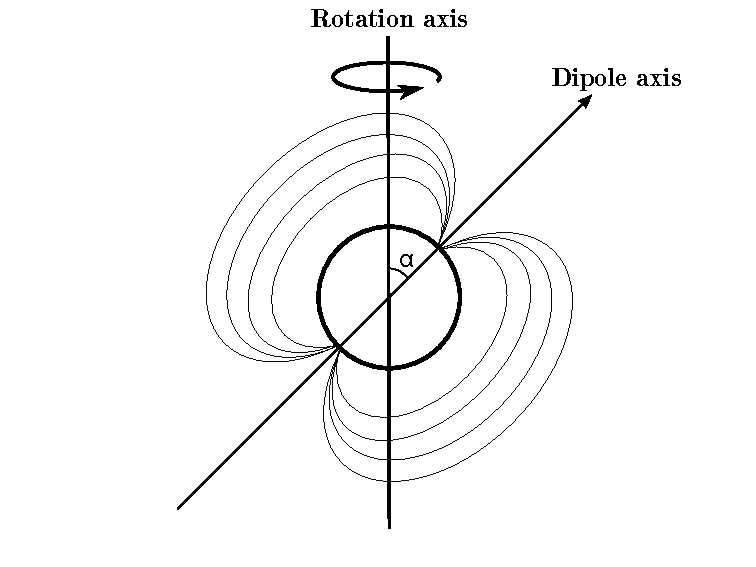
\includegraphics[width=.5\textwidth]{DipoleModelSimple}
    \caption{An illustration of the dipole spin-down model. The dipole and some 
    of the closed field lines are fixed at an angle $\alpha$ to the rotation 
    axis. As the body rotates, radiation is emitted along both ends of the dipole
    axis producing a torque on the body.}
    \label{fig: DipoleSpindownSimple}
\end{figure}

From \citet{Landau2013classical} the total radiation from a dipole rotated at
angular frequency $\Omega$ is given by
\begin{align}
I = \frac{2}{3}\frac{\Omega^{4}}{c^{3}} d_{0}^{2},
\end{align}
where $d_0$ is the projection of the dipole moment on the plane perpendicular
to the axis of rotation \citep{Pacini1967}. Following \citet{Shapiro83}, the
magnitude of the magnetic dipole moment for a star with radius $R$ and surface magnetic
field strength $B_0$ is $B_{0}R^{3}/2$. Including the projection onto the
plane perpendicular to the rotation axis, the total radiation is then
\begin{align}
I = \frac{1}{6}\frac{\Omega^{4}}{c^{3}} B_0^2 R^{6} \sin^{2}\alpha.
\end{align}

The rotational energy of a body spinning at $\Omega$ with a moment of inertia
$I_{0}$ is given by
\begin{equation}
    E = \frac{1}{2}I_{0}\Omega^{2}.
\end{equation}
Differentiating this expression with respect to time gives the loss of rotational
energy, $\dot{E}=I_0 \Omega\dot{\Omega}$. Assuming that all the energy is lost
to the rotation of the dipole, hence the name rotation powered pulsars, we can
equate $\dot{E} = -I$. We then rearrange
to give a power-law relation between the spin-down rate and the spin-frequency:
\begin{align}
\dot{\Omega} = -\frac{B_0^{2} R^{6} \sin^{2}\alpha}{6 c^{3} I_0} \Omega^{3}.
\end{align}

This power-law dependence is a model specific version of a more general
phenomenological power-law braking model
\begin{equation}
    \dot{\Omega} = -k \Omega^{n}.
    \label{eqn: power law spin-down}
\end{equation}
Generalising in this way suggests a powerful method to determine the type of
braking for a given pulsar. Specifically, differentiating Eqn.~\eqref{eqn: power law spin-down}
and rearranging it can be shown that
\begin{equation}
    n = \frac{\ddot{\Omega}\Omega}{\dot{\Omega}^{2}}.
    \label{eqn: measured braking index}
\end{equation}
Therefore, if $\ddot{\Omega}$ can be measured, then $n$ can be determined, and
hence used to infer the type of braking. For example, measuring $n=3$ would
indicate the pulsar braking is dominated by losses due to the magnetic dipole,
in contrast, it can be shown that gravitational wave braking would produce
$n=5$ \citep{Shapiro83}. Unfortunately, in reality, pulsars do not constrain this
value. Braking indexes have been measured with values as large as $\sim10^{6}$.
We will return to this issue in Sec.~ \ref{sec: evidence from anomalous braking
indices}.

To infer the age of the pulsar, Eqn.~\eqref{eqn: power law spin-down} can
be integrated between the initial values ($t=0, \Omega=\Omega_{i}$) and the
observed value ($\Omega_{\mathrm{o}}$) to give
\begin{equation}
    t = \frac{1}{(1-n)} \frac{\Omega_{\mathrm{o}}}{\dot\Omega_{\mathrm{o}}} 
        \left(1 - \frac{\Omega_{\mathrm{o}}^{n-1}}{\Omega_{i}^{n-1}}\right).
\label{eqn: characteristic age}
\end{equation}
Typically, we make the assumption that all
pulsars, regardless of their measure braking index, are dominated by EM braking
such that $N=3$. Then additionally assuming that $\Omega_{i} \gg
\Omega_{\mathrm{o}}$ we can approximate to a characteristic age
\begin{equation}
    \tau_c = \frac{-1}{2}\frac{\Omega_{\mathrm{o}}}{\dot\Omega_{\mathrm{o}}}
         = \frac{1}{2}\frac{P}{\Pdot},
\end{equation}
where $P=\frac{2\pi}{\Omega}$ is the pulse period and
$\dot{P}=-2\pi\frac{\dot{\Omega}}{\Omega^{2}}$ is the period derivative.

To infer the approximate surface magnetic field strength, we first note that
in the EM dipole braking model:
\begin{align}
k = \frac{B_0^{2} R^{6} \sin^{2}\alpha}{6c^{3}I_0}.
\end{align}
Then rearranging and substituting for $k$ in Eqn.~\eqref{eqn: power law
spin-down} we can estimate the surface magnetic field strength by
\begin{equation}
    B_{0} = \left(\frac{6 c^{3} I_{0}}{R^{6} \sin^{2}\alpha}\right)^{\frac{1}{2}} 
            \left(\frac{-\dot{\Omega}}{\Omega^{3}}\right)^{\frac{1}{2}}
          = \frac{1}{2\pi}\left(\frac{6 c^{3} I_{0}}{R^{6} \sin^{2}\alpha}\right)^{\frac{1}{2}}
           \sqrt{P \Pdot}
\label{eqn: surface magnetic field}
\end{equation}
In general we do not know the inclination angle $\alpha$, but we can evaluate a 
minimum magnetic field strength by setting $\alpha=\pi/2$. In CGS units, for a
canonical pulsar with $R=10^{6}$~cm, $I_{0}=10^{45}$~g~cm$^{2}$ \citep{Lyne2012book}, we can approximate
the magnetic field strength as
\begin{equation}
    B_{0} = 3.2 \times 10^{19} \sqrt{P \Pdot}.
\label{eqn: surface magnetic field canonical}
\end{equation}

In this section, we have introduced some of the simple results that can be
obtained by modelling the time evolution of pulsars with a power law. In
practise this model is consisent with most pulsar observations and provides a
useful way to categorise them via their spin-down age and magnetic field.
However, such a model does not capture all of the subtle variations which are
the focus of this thesis.  We will frequently refer back to this model as it
provides a useful platform from which to begin understanding neutron stars.



\FloatBarrier
%\section{The importance of neutron stars}
%%Neutron stars fill an important role in fundamental physics. Their extreme
%%densities but low temperatures make then ideal laborotories to explore this
%%region of the QCD phase diagram. In particular the study of the equation of
%%state at nuclear densities. Their extreme compactness 
%
%\section{Neutron stars as a source of gravitational waves}

\section{Pulsar timing methods}
\label{sec: pulsar timing methods}
Pulsars can be observed by measuring the variation in amplitude of the radio
waves from a particular sky location. A single observation consists of
measuring the amplitude over a time period of approximately $30$ minutes or so,
which, for pulsars with spin period~$\sim1$~s, means recording up to several
thousand individual pulsations.

The shape of individual pulses can vary substantially during a single
observation; to demonstrate this, in Figure~\ref{fig: CP1919 stacked},
successive pulses from PSR~B1919+21, the first discovered pulsar, are
vertically stacked and aligned.
\begin{figure}[htb]
\centering
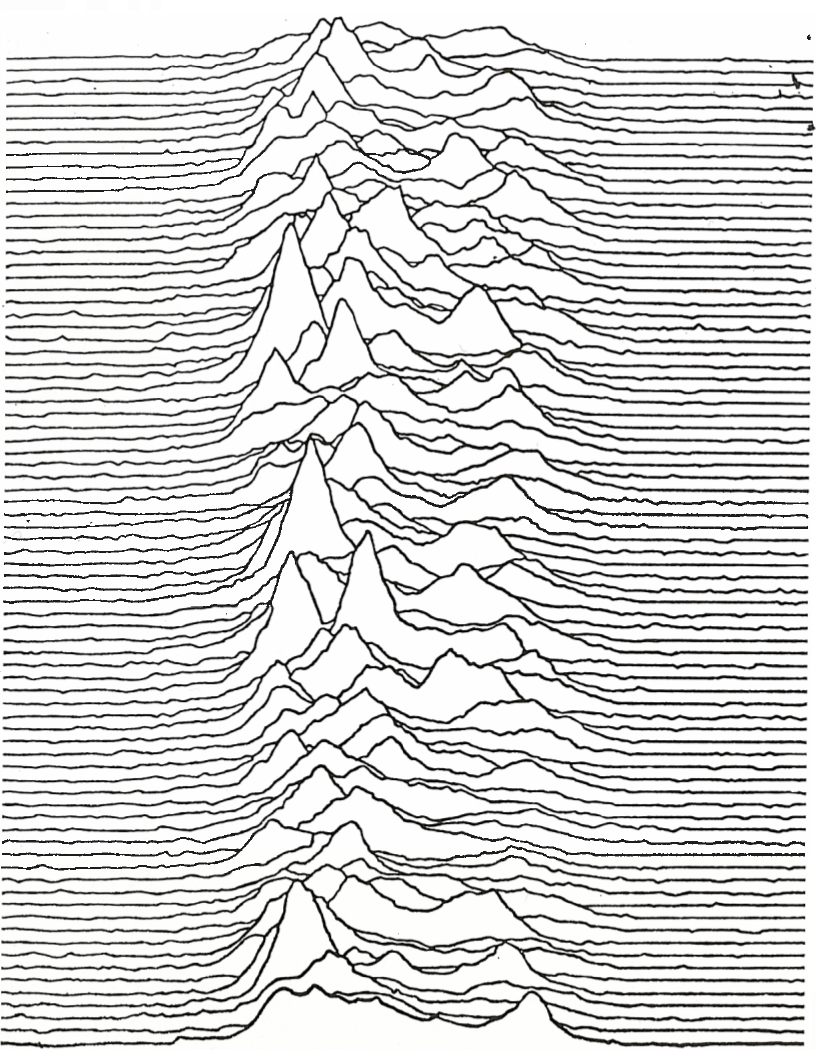
\includegraphics[width=0.5\textwidth]{CP1919_stacked}
\caption{The radio amplitude of successive pulses from PSR~B1919+21 stacked
vertically, figure reproduced from \citet{mitton1977cambridge}, originally
produced by \citet{craft1970}.}
\label{fig: CP1919 stacked}
\end{figure}
Each pulsation lasts for a small fraction of the pulse period. As an example,
the pulses in PSR~B1919+21, shown in Figure~\ref{fig: CP1919 stacked}, have
typical widths of $0.031$~s, but the pulse period is $1.337$~s; note that the
stacked plot is truncated to show only the pulsation itself. Later, in
Figure~\ref{fig: pop stats others}, we will show this to be a common
characteristic for the normal radio pulsar population by looking at the
duty-cycle, the ratio of the pulse duration to the pulse period.

In order to understand the gross features of a pulsar, astronomers average over
the hundreds to thousands of pulses observed during a single observation to
create a single integrated pulse profile. This is done by sampling the radio
signal at fixed time intervals then `folding' all the samples at the pulse
period (for a complete review see \citet{Lyne2012book}). In contrast to the
individual pulses which, as shown in Figure~\ref{fig: CP1919 stacked}, can be
highly variable, the integrated pulse profile is highly stable between
independent observations over timescales of years.

The integrated pulse profile not only gives a stable picture of what the
pulsations look like on average, but it also provides a highly accurate
measurement of the time of arrival (TOA) of a single pulse during the
observation. It is this TOA
which can be used to `time' a pulsar. To do this, regular observations of a
pulsar must be made every few months or so, with each observation resulting in a
precise TOA measurement. Having obtained a series of TOAs, pulsar astronomers
generate a \emph{timing model} which attempts to exactly count each and every
pulse. Between any two observations there may be several million pulses so the
timing model needs to account for any mechanisms which may produce variations
in the TOAs.  The process is standardised by the software package
\texttt{TEMPO2} developed by \citet{Hobbs2006}, of which we will now describe the
essential features.

The TOA of a pulse at the detector on Earth depends on many factors, such as: the
time at which the beam was directed by the source towards the Earth; the relative
motions of the source and detector; and any mechanisms effecting the signal during
its transit. In this thesis, we will be concerned only with the time at which
pulses are generated (when the source beams towards
the earth) which is governed by the \emph{timing properties} of the star itself.
As described by \citet{Edwards2006} these can be modelled by a Taylor expansion
in the phase at time $t$, given by
\begin{equation}
\phi(t) = \phi_0 + 2\pi \sum_{n\ge 1}\frac{\nu^{(n-1)}}{n!}(t - \tref)^{n},
\label{eqn: Taylor compact}
\end{equation}
where $\{\nu^{(n)}\}$ is the $n^\mathrm{th}$ time derivative of the spin
frequency of the rotating body, $\phi_0$ is the initial phase, and
$\tref$ is an arbitrary reference time. This expansion is usually truncated at
$n=3$, the second order spin-down rate $\ddot{\nu}$. The timing model then
includes corrections to this to model the relative motion of the source and
detector, intergalactic transit, and other effects; these are described in full
in \citet{Edwards2006}.

Between any two TOAs, if the timing model is correct, an integer number of
rotations must have occurred; this allows the use of the deviation of
$\phi(t_{TOA}^{j})$ from an integer as a test statistic. The timing model
minimises the root-mean-square (RMS) of these deviations with respect to the timing model
parameters, for example the frequency and frequency derivatives. The output of
applying a particular timing model (choice of corrections) to a set of data is
then the best-fit of these parameters and an estimate of their associated
errors.  The corrections applied in a timing model provide a method to
investigate pulsar physics: for example in some pulsars an orbital correction
must be applied which models the periodic motion of the star due to an orbital
companion. Using this technique, \citet{wolszczan1992planetary} discovered the
first \emph{exoplanets} orbiting the pulsar PSR~B1257+12.

A minimisation of the timing model parameters will converge regardless of
whether of not the model itself is appropriate. To qualitatively check if the
fitted model described the data, pulsar astronomers refer to the \emph{timing
residual}, which is the difference between the TOA, as given by the timing
model, and the actual TOA. The timing residual provides a mechanism to evaluate
the timing model: for example a periodic variation in the timing residual with period
$365$~days may indicate the correction of the Earth's orbit about the Sun may
be incorrect. If the timing model is correct, the residual data points should
be Gaussianly distributed around zero. A timing model is described as
\emph{phase-connected} if it is accurate enough to track the pulsar to within a
single rotation. For most pulsars this is the case and a single set of
coefficients can track the spin-down over periods greater than a year.

However, for all pulsars the timing residual contains `structure' known as
\emph{timing variations} which cannot be associated with any known correction.
These variations are the focus of this work and we will describe the details
further in Section~\ref{sec: timing variations}.  In the next section, we will
describe the variety of known pulsars which have been timed using this method.




\section{Glitches}
\label{ref: glitches}
In addition to the regular spin-down of radio pulsars due to magnetic braking, some
pulsars undergo anomalies in their timing solutions known as \emph{glitches}.
\citet{Edwards2006} describes how these can be modelled by a permanent increase
in the phase, frequency, and first frequency derivative in addition to a
frequency increment that subsequently decays exponentially to zero. That is,
Eqn.~\eqref{eqn: Taylor compact} picks up an additional term
\begin{align}
\phi_{\textrm{g}} = \left\{
\begin{array}{ll}
\Delta\phi + \Delta\nu(\tTOA - \tg) + \frac{1}{2}\Delta\dot{\nu}(\tTOA - \tg)^{2}
+ \left[1-\textrm{e}^{-(\tTOA - \tg)/\tau}\right]\Delta\nu_{\textrm{t}}(\tTOA - \tg)
& \tTOA \ge \tg \\
0 & \tTOA < \tg
\end{array}
\right.
\label{eqn: glitch timing model}
\end{align}
for each modelled glitch. The first three terms are the permanent increase
in phase, frequency, and spin-down, while the last term gives the transient
increase in the frequency $\Delta\nu_{\textrm{t}}$ which decays exponentially
with a timescale $\tau$. In effect this means that pulsar astronomers fit
separate a Taylor expansions either side of the glitch. Due to the fact that
the rise time over which glitch occurs is short compared to the frequency
with which observers take measurements, timing solutions can not resolve the
detailed variation which occur during the glitch: they are limited to describing
the global behaviour before and after.

Fitting this model, pulsar astronomers find that glitches are sudden positive
jumps in the frequency $\Delta\nu > 0$, with typical values of $10^{-9}$~Hz to
$10^{-4}$~Hz; for some pulsars this is accompanied by a change, with either
sign, in the spin-down which has absolute magnitudes between $10^{-19}$~Hz/s to
$10^{-12}$~Hz/s. A comprehensive review of glitches was carried out by
\citet{Espinoza2011} and to illustrate a typical glitch we present a figure
from this work in Fig.~\ref{fig: glitch}.
\begin{figure}[htb]
    \centering
    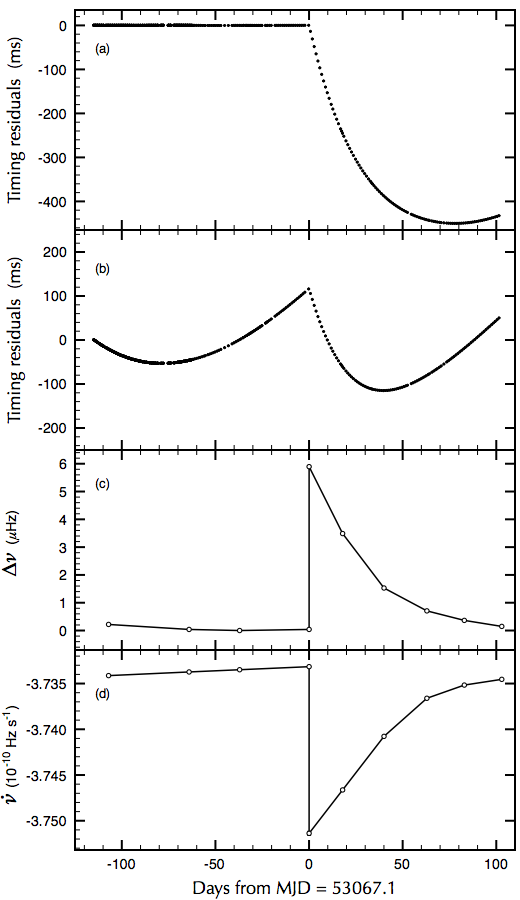
\includegraphics[width=0.5\textwidth]{GlitchExample_jbman}
    \caption{
A glitch in the data of PSR B0531+21, the Crab pulsar. It occurred around MJD
53067 and had a fractional frequency jump of $\Delta\nu/\nu = 5.33 \pm 0.05
\times 10^{−9}$; a small glitch. (a) The timing residuals relative to a
slowdown model with two frequency derivatives when fitting data only up to the
glitch date. (b) Timing residuals after fitting all data in the plot; note
that the glitch feature is still visible. Both these panels have the same
scale, cov- ering 500 ms. (c) Frequency residuals, obtained by subtracting the
main slope given by an average $\dot\nu$.  (d) The behaviour of $\dot\nu$
through the glitch. This figure and caption are taken from Fig.~1 of
\citet{Espinoza2011}}
    \label{fig: glitch}
\end{figure}

Eqn.~\eqref{eqn: glitch timing model} models the glitch with a so-called recovery
consisting of a fraction $Q$ of the initial frequency jump which decays over
a timescale $\tau$ leaving only the permanent increase in frequency. A review
including measurements of this was conducted by \citet{Lyne2000}; they found
that in glitches from 18 pulsars, $Q$ correlates with $|\dot{\nu}|$ reaching
values as large as $\sim0.9$ for the youngest pulsar with the highest absolute
spin-down rate, PSR~B0531+21 also known as the Crab pulsar.

Many pulsars have been observed to glitch several times, \citet{Melatos2008}
considered the waiting times between glitches and concluded that in most
glitching pulsars the glitches happen randomly with waiting times consistent
with a Poisson process, except in PSR J0537-6910 and PSR J0835-4510 which
displayed quasi-periodicity in the waiting times.

In Chapter~\ref{sec: glitches in cgw} we perform our own investigation into the
population statistics of glitches with an aim to understand their implication
for gravitational wave searches. We find, in agreement with
\citet{Espinoza2011} and references therein, that the distribution of glitch
magnitudes has multiple modes which suggests that glitches may come from more
than one mechanism. We go on to apply a statistical model and determine, in an
empirical fashion, the properties of the underlying source populations.

Glitches provide a unique opportunity to investigate the physics of neutron
stars and many of the leading insights have been gained by their study. Two
leading models exist known as the \emph{superfluid unpinning} model and the
\emph{starquake} model.

In the superfluid unpinning model proposed by \citet{Anderson1975}, the star
contains a superfluid component in which the angular momentum is stored in an
array of vortices which are `pinned' to the crust. The magnetic dipole is
frozen into the crust and exerts a torque on the crust, gradually spinning it
down. The superfluid component cannot decrease its angular momentum without
destroying its vortices and so does not spin-down at the same rate.  A lag in
frequency between the superfluid component and rest of the crust develops until
the forces are sufficiently large to cause an avalanche of unpinning events
rapidly transferring the stored angular momentum in the superfluid component to
the crust. The observed pulsations measure the rotation rate of the crust into
which the dipole is frozen, so when this unpinning occurs, we see a rapid
increase in the frequency.

The second model, starquakes, follows from the observation that a rapidly
spinning fluid body has an oblate `rest shape' with a bulge about its equator
due to the centrifugal force. The crust of a star spinning at a frequency $\nu_0$
will solidify with a corresponding oblateness. Subsequently, as the star spins down,
it will have a different rest shape due to its decreased frequency, but the crust
will retain a memory of the earlier shape at which it solidified. This will cause
strains in the crust which eventually cause a starquake relieving the strain,
resetting the reference rest shape, and producing glitch like features.

Both of these models have support in the literature and have been developed
significantly to explain the variety of observed glitches. However, there are
observations which cause difficulties for both models: glitches seen in the
Vela pulsar are too large and too often to be consistent with a starquakes
model, while the unpinning model requires a superfluid component which is at
odds with observation of precession (we discuss this further in
Chapter~\ref{sec: testing models}).




\FloatBarrier
\section{Timing noise}
\label{sec: timing noise}
Timing noise refers to small, low level structure in the timing residual which
cannot be attributed to any other source, an example is given in figure
\ref{fig: timing noise example}. The amount of timing noise will depend on the
order of truncation of the Taylor expansion.  In most studies, and so in this
work, we will truncate at $n=3$, the second order spindown; the timing noise is
then the residual left after a $n=3$ fit. Increasing this truncation level can
fit out these variations, but we are interested in understanding the origins
and implications of timing noise.

\begin{figure}[htb] 
    \centering
    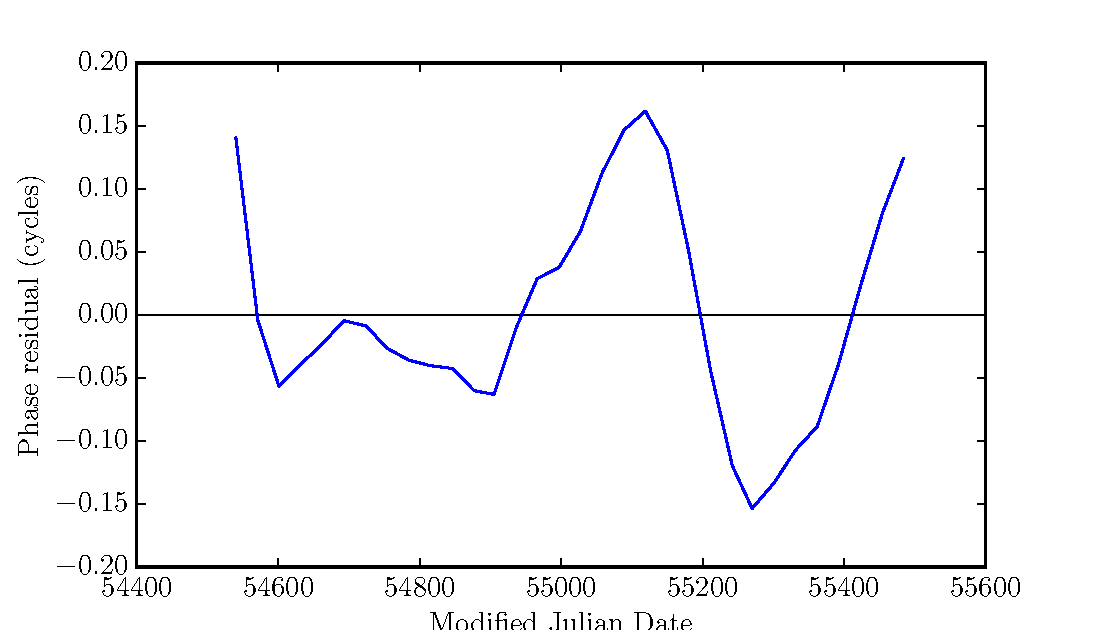
\includegraphics[width=0.75\textwidth]{Crab_residual_phase}
    \caption{A timing residual demonstrating structure which is named timing
        noise.  This is generated from data on the Crab ephemeris (see section
    \ref{sec: timing noise as described by the crab ephemeris})}
    \label{fig: timing noise example}
\end{figure} 

There have been various attempts to characterise timing noise
over the history of 
pulsar astronomy. Most observations are tied to a particular interpretation
which we will discuss in part \ref{sec: interpretations of timing noise}.
It is however worth first listing some of the model independent observations.
These are summarised by the most comprehensive study of timing noise from 
\citet{Hobbs2010} who considered 366 pulsars over time scales $\gtrsim10$~years.
They found that:
\begin{enumerate}

    \item Timing noise is widespread in pulsars

    \item Timing noise is inversely correlated the characteristic age
        defined in equation \ref{eqn: characteristic age}

    \item The structures seen in the timing residual vary with data span. As
        more data is collected, more quasi-periodic features are observed.

    \item The dominant contribution to timing noise for young pulsars with
        $\tau_{c}<10^{5}$~years can be explained as being caused by the
        recovery from previous glitches.

    \item A handful of pulsars exhibit significant periodicity's while
        quasi-periodicity's are observed in many pulsars

\end{enumerate}




\biblio


\end{document}
